%% =====================================================================
%%  Technical report - A Visual Study of E-Commerce Orders,
%%  Delivery and Customer Satisfaction
%%
%%  Build:  tectonic technical_report.tex
%%     or:  latexmk -pdf technical_report.tex
%%
%%  Figures are read from ./figures/, which is produced by
%%  `make figures` in the project root. Every number quoted in the prose
%%  comes from outputs/tables/ and is reproducible with `make all`.
%% =====================================================================
\documentclass[11pt,a4paper]{article}

\usepackage[T1]{fontenc}
\usepackage[utf8]{inputenc}
\usepackage{lmodern}
\usepackage{microtype}
\usepackage[english]{babel}

\usepackage[margin=2.4cm,top=2.6cm,bottom=2.6cm]{geometry}
\usepackage{graphicx}
\usepackage{booktabs}
\usepackage{longtable}
\usepackage{array}
\usepackage{caption}
\usepackage{float}
\usepackage{enumitem}
\usepackage{xcolor}
\usepackage{fancyhdr}
\usepackage{titlesec}
\usepackage{listings}
\usepackage{amsmath}
\usepackage[hidelinks]{hyperref}

% assets/ holds the logo. It deliberately does not live in figures/, because
% `make clean` wipes reports/figures/* and would delete it.
\graphicspath{{figures/}{assets/}}

%% ---- project palette, matching the dashboard and the figures ----------
\definecolor{navy}{HTML}{1F3A68}
\definecolor{amber}{HTML}{E8833A}
\definecolor{ink}{HTML}{2B3245}
\definecolor{muted}{HTML}{6B7488}
\definecolor{rule}{HTML}{E6E9EF}
\definecolor{wash}{HTML}{F7F9FC}
\definecolor{good}{HTML}{2E8B6F}
\definecolor{bad}{HTML}{C1462F}

\hypersetup{colorlinks=true,linkcolor=navy,urlcolor=navy,citecolor=navy}

%% ---- headings ---------------------------------------------------------
\titleformat{\section}{\normalfont\Large\bfseries\color{navy}}{\thesection}{0.7em}{}
\titleformat{\subsection}{\normalfont\large\bfseries\color{ink}}{\thesubsection}{0.7em}{}
\titleformat{\subsubsection}{\normalfont\normalsize\bfseries\color{ink}}{\thesubsubsection}{0.7em}{}
\titlespacing*{\section}{0pt}{2.2ex plus 1ex minus .2ex}{1.2ex plus .2ex}

\pagestyle{fancy}
\fancyhf{}
\renewcommand{\headrulewidth}{0.4pt}
\fancyhead[L]{\small\color{muted}Orders, Delivery and Customer Satisfaction}
\fancyhead[R]{\small\color{muted}Technical Report}
\fancyfoot[C]{\small\color{muted}\thepage}

\captionsetup{font=small,labelfont={bf,color=navy},width=0.92\textwidth}

%% ---- code listings ----------------------------------------------------
\lstdefinestyle{py}{
  language=Python,
  basicstyle=\ttfamily\footnotesize,
  keywordstyle=\color{navy}\bfseries,
  commentstyle=\color{muted}\itshape,
  stringstyle=\color{good},
  numbers=left, numberstyle=\tiny\color{muted}, numbersep=8pt,
  frame=single, rulecolor=\color{rule},
  backgroundcolor=\color{wash},
  breaklines=true, breakatwhitespace=true,
  showstringspaces=false,
  xleftmargin=14pt, framexleftmargin=14pt,
  captionpos=b,
}
\lstset{style=py}

%% ---- a callout box for key findings -----------------------------------
\newcommand{\finding}[1]{%
  \par\vspace{0.6em}%
  \noindent\begin{minipage}{\textwidth}%
  \setlength{\fboxsep}{9pt}%
  \noindent\colorbox{wash}{\begin{minipage}{\dimexpr\textwidth-2\fboxsep\relax}%
  \color{ink}\textbf{#1}%
  \end{minipage}}%
  \end{minipage}\par\vspace{0.6em}%
}

\newcommand{\R}{R\$}

\begin{document}

%% ======================================================== title page
\begin{titlepage}
\centering
\vspace*{2.2cm}
% Plain \includegraphics, not a figure environment: a float inside titlepage
% has nowhere to anchor and LaTeX defers it to a later page.

\includegraphics[width=0.20\textwidth]{iitm_logo.png}\\[1.6em]
{\color{amber}\large\bfseries DATA VISUALIZATION AND DESIGN PROJECT}\\[0.5em]
{\color{navy}\Huge\bfseries E-Commerce Orders, Delivery\\[0.35em] and Customer Satisfaction}\\[1.4em]

{\color{ink}\large Growing a marketplace without breaking the customer experience}\\[2.4em]

\textcolor{rule}{\rule{0.35\textwidth}{1.2pt}}\\[2.2em]

{\large\bfseries\color{navy}Technical Report}\\[2.6em]

\begin{tabular}{@{}ll@{}}
\toprule
\multicolumn{2}{@{}l}{\bfseries\color{navy}Project Team - 12}\\
\midrule
1. \lbrack 23f1002398@ds.study.iitm.ac.in\rbrack& KARTHIK BALAJI SIRIMILLA\\
2. \lbrack 23f1002849@ds.study.iitm.ac.in\rbrack& CALEB KUMAR PALLAPU\\
3. \lbrack 22f3002812@ds.study.iitm.ac.in\rbrack& MOHD HASHIR\\
4. \lbrack 24f2005934@ds.study.iitm.ac.in\rbrack& KAUTILYA SAGILI\\
5. \lbrack 22f1001943@ds.study.iitm.ac.in\rbrack& JEEVAN RAMKRISHNA CHOUDHARY\\
\bottomrule
\end{tabular}

\vspace{2.2em}
{\color{muted}\small
Submission date: \lbrack 11-Sep-2026\rbrack}

\vfill
{\color{muted}\small
Dataset: Brazilian e-commerce public dataset (99{,}441 orders, Sept 2016 -- Oct 2018),\\
combined with the associated marketing funnel tables.}
\end{titlepage}

%% ======================================================== abstract
\section*{Executive summary}
\addcontentsline{toc}{section}{Executive summary}

Leadership at the marketplace wants to grow the seller base without degrading the
customer experience and believes the two are in tension. This study tests that
belief against 99{,}441 orders and finds it is only half right. Growth and
experience are not opposed across the business; they are opposed in a small
number of identifiable places and most of those cost far less to fix than the
framing of the problem assumes.

Three findings drive the recommendations. First, late delivery is overwhelmingly
the dominant driver of dissatisfaction: orders delivered on time average 4.30
stars, orders delivered late average 2.57. Second, that damage is not gradual.
Delivering an order fifteen days early scores no better than delivering it two
days early, while delivering five to ten days late collapses the average to 1.89.
The correct operational target is therefore the tail of the distribution, not the
mean. Third and contrary to the framing we were given, most of the delay does not
belong to the sellers. Sellers hand parcels to the carrier in 2.8 days on average;
the carrier then holds them for 9.3 days and carrier transit correlates with the
review score roughly twice as strongly as seller handling does.

We quantify where risk concentrates using a purpose-built metric, Satisfaction-at-Risk,
which weighs a segment's severity by its size. We then price five candidate
interventions by replaying the real order history with each lever applied. Only one
improves customer experience at no revenue cost: targeted investment in carrier
speed on the worst-performing lanes, of which S\~{a}o Paulo to Rio de Janeiro is by
some distance the largest. One intervention that appears obviously attractive,
tightening the quoted delivery promise is shown to be actively harmful.

All analysis is reproducible from the raw CSV files with a single command. The
accompanying repository contains the pipeline, three narrative notebooks and an
interactive dashboard, all reading from one shared analysis layer.

\vspace{1em}
\newpage
\tableofcontents
\newpage

%% ======================================================== 1
\section{Introduction}

\subsection{Business context}

The marketplace connects several thousand small and medium sellers to customers
distributed across Brazil and provides the logistics layer that moves goods
between them. Its commercial goal is growth in gross merchandise value (GMV),
which is driven primarily by recruiting sellers and expanding the catalogue.

The tension that motivates this study is straightforward to state. Onboarding
sellers aggressively raises gross sales, but introduces sellers who deliver
late or sell poorly rated products and dissatisfied customers do not return.
Conversely, policing every underperforming seller improves average quality but
shrinks the catalogue and slows growth. Both statements are true, which is why the
trade-off feels unavoidable and why the decisions are currently being made on
judgement rather than evidence.

\subsection{Objectives}

We translated the business goal into five analysis questions, chosen because each
one is answerable from the available data and each one changes a decision:

\begin{enumerate}[leftmargin=*,itemsep=0.25em]
  \item Is the marketplace already trading satisfaction for growth or is it only at
        risk of doing so?
  \item What actually drives a one-star review: the product, the seller or the
        delivery?
  \item If delivery, which part of the journey is responsible, seller handling
        or carrier transit?
  \item Which categories, regions, shipping lanes and sellers carry
        disproportionate risk?
  \item What would each available intervention cost in revenue and buy in
        goodwill?
\end{enumerate}

Questions 1 through 3 establish causality and magnitude. Question 4 localizes the
problem so that an intervention can be targeted. Question 5 converts the analysis
into a decision.

\subsection{Scope and deliverables}

The project produced four artifacts: a reproducible data pipeline, three narrative
notebooks documenting the analysis week by week, an interactive dashboard and this
report. Section~\ref{sec:appendix} documents the code in detail.

%% ======================================================== 2
\section{Data}

\subsection{Sources}

The primary dataset comprises nine relational tables describing the complete
purchase journey, supplemented by two marketing tables describing seller
acquisition. Table~\ref{tab:tables} summarises each.

\begin{table}[H]
\centering
\small
\caption{The eleven source tables and the grain of each.}
\label{tab:tables}
\begin{tabular}{@{}p{3.1cm}p{2.0cm}p{9.4cm}@{}}
\toprule
\textbf{Table} & \textbf{Grain} & \textbf{Contents}\\
\midrule
orders & one order & Lifecycle timestamps: purchase, payment approval, carrier
handoff, customer delivery and the estimated delivery date quoted at checkout.\\
order\_items & one item & Price, freight, product and seller. An order may contain
several items from several sellers.\\
order\_payments & one payment & Method, instalment count, value.\\
order\_reviews & one review & A 1--5 star score and an optional free-text comment.\\
customers & one order & Delivery location. Note that \texttt{customer\_id} is minted
per order; \texttt{customer\_unique\_id} identifies the person.\\
sellers & one seller & Seller location.\\
products & one product & Category, weight, dimensions, photo count.\\
category\_translation & one category & Portuguese to English category names.\\
geolocation & one zip prefix & Sampled coordinates, used to estimate distance.\\
mql & one lead & Marketing-qualified leads entering the seller funnel.\\
closed\_deals & one deal & Leads that converted into registered sellers.\\
\bottomrule
\end{tabular}
\end{table}

\subsection{Grain and join hazards}

Establishing the grain of each table before joining anything is not a formality.
Three properties of this schema will silently corrupt results if missed:

\begin{itemize}[leftmargin=*,itemsep=0.3em]
  \item \textbf{\texttt{order\_items} has more rows than \texttt{orders}.} Any
        order-level measure must be aggregated first. ``Number of orders'' and
        ``number of items'' are different questions with different answers.
  \item \textbf{\texttt{order\_reviews} contains duplicate orders.} 547 orders
        were surveyed more than once. A naive join duplicates those orders and
        over-weights them; because re-surveying correlates with dissatisfaction,
        the bias is not random.
  \item \textbf{\texttt{customer\_id} is not a person.} A fresh identifier is
        generated per order, so counting distinct \texttt{customer\_id} values
        yields the order count. The repeat-purchase rate, on which the entire
        valuation argument in Section~\ref{sec:sar} rests, is only computable
        from \texttt{customer\_unique\_id}.
\end{itemize}

%% ======================================================== 3
\section{Data preparation}

\subsection{Quality audit}

The ingest stage walks every table looking for missing values, internal
contradictions and physically impossible events. Each finding is recorded
alongside the treatment applied, so that the judgement calls are auditable rather
than buried in code. Table~\ref{tab:audit} lists the material findings.

\begin{table}[H]
\centering
\small
\caption{Data quality findings and treatments. Shares are of the relevant table.}
\label{tab:audit}
\begin{tabular}{@{}p{5.6cm}rp{7.4cm}@{}}
\toprule
\textbf{Finding} & \textbf{Rows} & \textbf{Treatment}\\
\midrule
No delivery date recorded & 2{,}965 & Retained, but excluded from any metric
requiring the delivery outcome.\\
Status ``delivered'' with no delivery date & 8 & Dropped from delivery analysis:
the outcome date is unknowable.\\
Lifecycle timestamps out of order & 1{,}382 & Order retained; the impossible stage
duration is nulled so it cannot distort stage averages.\\
Order surveyed more than once & 547 & Earliest review per order retained.\\
Product category missing & 610 & Mapped to \texttt{unknown} rather than dropped,
so the orders survive the join.\\
Review with no written comment & 58{,}247 & Text analysis runs on the commented
subset only; stated as a caveat.\\
Closed deals whose seller never transacted & 462 & Funnel analysis scoped to
matched sellers; the gap is reported, not hidden.\\
\bottomrule
\end{tabular}
\end{table}

\subsection{Two decisions that would have changed the answer}

Most treatments above are routine. Two were not and both are the kind of default
that produces a confidently wrong result.

\paragraph{Lateness must be unknown, not false.} When an order has no delivery
date, the question ``was it late?'' has no answer. The convenient default is
\texttt{False} and it is wrong: it silently classifies every undelivered order as
on time and inflates the on-time rate. We represent it as null throughout and
every rate reported in this document is computed only over orders where the
question has an answer.

\paragraph{Null the impossible stage, not the order.} 1{,}382 orders carry
timestamps that run backwards, which are recording artefacts rather than events.
Discarding those orders would remove 1.4\% of the data; the purchase-to-delivery
duration remains valid for them and only the individual stage is meaningless. We
therefore null the offending stage duration and retain everything else, which costs
one field on 1.4\% of orders rather than 1.4\% of the dataset.

\subsection{The analysis population}

Every satisfaction statistic in this report is computed on the same set of orders:
\textbf{delivered and carrying a review}, restricted to January 2017 through
August 2018. The date window is trimmed because the months on either side contain
too few orders to support a monthly trend. This population is defined once, in a
single function, so that no two figures in the project can disagree about their
denominator.

\begin{table}[H]
\centering
\small
\caption{From raw data to analysis population.}
\label{tab:population}
\begin{tabular}{@{}lrr@{}}
\toprule
& \textbf{Orders} & \textbf{Share}\\
\midrule
Raw orders & 99{,}441 & 100.0\%\\
Delivered, reviewed, within the reporting window & 95{,}560 & 96.1\%\\
\midrule
Of which delivered late & 7{,}658 & 8.0\%\\
Of which received a 1--2 star review & 12{,}218 & 12.8\%\\
\bottomrule
\end{tabular}
\end{table}

\subsection{Feature construction}

The relational structure is convenient for storage and awkward for analysis, so it
is flattened into one row per order. The features that matter most decompose the
delivery journey into stages, because that is what assigns a delay to a
responsible party (Table~\ref{tab:stages}).

\begin{table}[H]
\centering
\small
\caption{Delivery journey decomposition.}
\label{tab:stages}
\begin{tabular}{@{}llll@{}}
\toprule
\textbf{Stage} & \textbf{From} & \textbf{To} & \textbf{Responsible party}\\
\midrule
Approval & purchase & payment cleared & payment system\\
Handling & payment cleared & carrier collects & \textbf{the seller}\\
Transit & carrier collects & customer receives & \textbf{the carrier}\\
\bottomrule
\end{tabular}
\end{table}

To these we add \texttt{delay\_days}, defined as the actual delivery date minus the
date promised at checkout. Positive values indicate lateness. This is deliberately
measured against the promise rather than against any objective standard, because
the promise is what the customer experiences: they do not know how long an order
``should'' take, only what they were told.

%% ======================================================== 4
\section{Methodology}

\subsection{Satisfaction-at-Risk}
\label{sec:sar}

Ranking segments by their average score is misleading, because it cannot
distinguish a small terrible segment from a large mediocre one. Maranh\~{a}o has a
poor average score across 709 orders; Rio de Janeiro is mid-table across 12{,}172.
Ranking by badness sends you to the first; ranking by size sends you to the second;
neither reflects total goodwill destroyed.

We therefore define, for any segment,
\begin{equation}
\text{excess detractors} = n \times (p_{\text{segment}} - p_{\text{marketplace}})
\end{equation}
where $n$ is the segment's order count and $p$ is its rate of 1--2 star reviews.
In plain terms: how many bad reviews would disappear if this segment merely behaved
like the marketplace average. A positive value identifies a segment destroying more
goodwill than its size warrants.

To express this in currency we multiply by the segment's average order value. That
step is a judgement call and rests on one observation: only 3.1\% of customers ever
place a second order. In a market with effectively no repeat purchase, a
dissatisfied customer is not someone to win back but someone already lost and the
acquisition spend behind them bought exactly one order. Valuing a detractor at one
average order value is therefore a defensible \emph{floor}. It ignores word of
mouth and the future orders never placed, so the true cost is higher; we prefer to
under-claim.

\subsection{Predictive modelling}

Two models are fitted, answering deliberately different questions. The
\emph{post-hoc} model includes the realised delivery outcome and answers what
explains a bad review. The \emph{at-risk} model uses only features knowable at
checkout and answers whether a bad review can be anticipated in time to intervene.

Two methodological constraints were imposed to prevent optimistic results:

\begin{itemize}[leftmargin=*,itemsep=0.3em]
  \item \textbf{Temporal split.} Training uses earlier orders and testing uses
        later ones. A random split allows the model to learn from future orders to
        predict past ones, which inflates every metric.
  \item \textbf{Strictly prior seller history.} A seller's lifetime average score
        cannot be used to predict an order that is itself part of that average. It
        is computed as an expanding mean shifted by one order.
\end{itemize}

The estimator is a gradient-boosted tree ensemble
(\texttt{HistGradientBoostingClassifier}) with ordinal-encoded categoricals.

\subsection{Scenario simulation}

Rather than assuming an effect size, we estimate the empirical relationship between
lateness and detractor probability directly from the data, constrain it to be
monotone and then replay the actual order history with each lever applied. Reading
the new detractor count off the fitted curve produces estimates that are honest
about their own precision: they are magnitudes suitable for ranking options against
each other, not forecasts suitable for budgeting to two decimal places.

%% ======================================================== 5
\section{Exploratory analysis}

\subsection{Growth is not visibly costing satisfaction}

GMV grows roughly tenfold across the reporting window while the average review
score remains near 4.16, ending slightly higher than it started
(Figure~\ref{fig:growth}). Taken at face value this suggests no problem exists.

\begin{figure}[H]
\centering
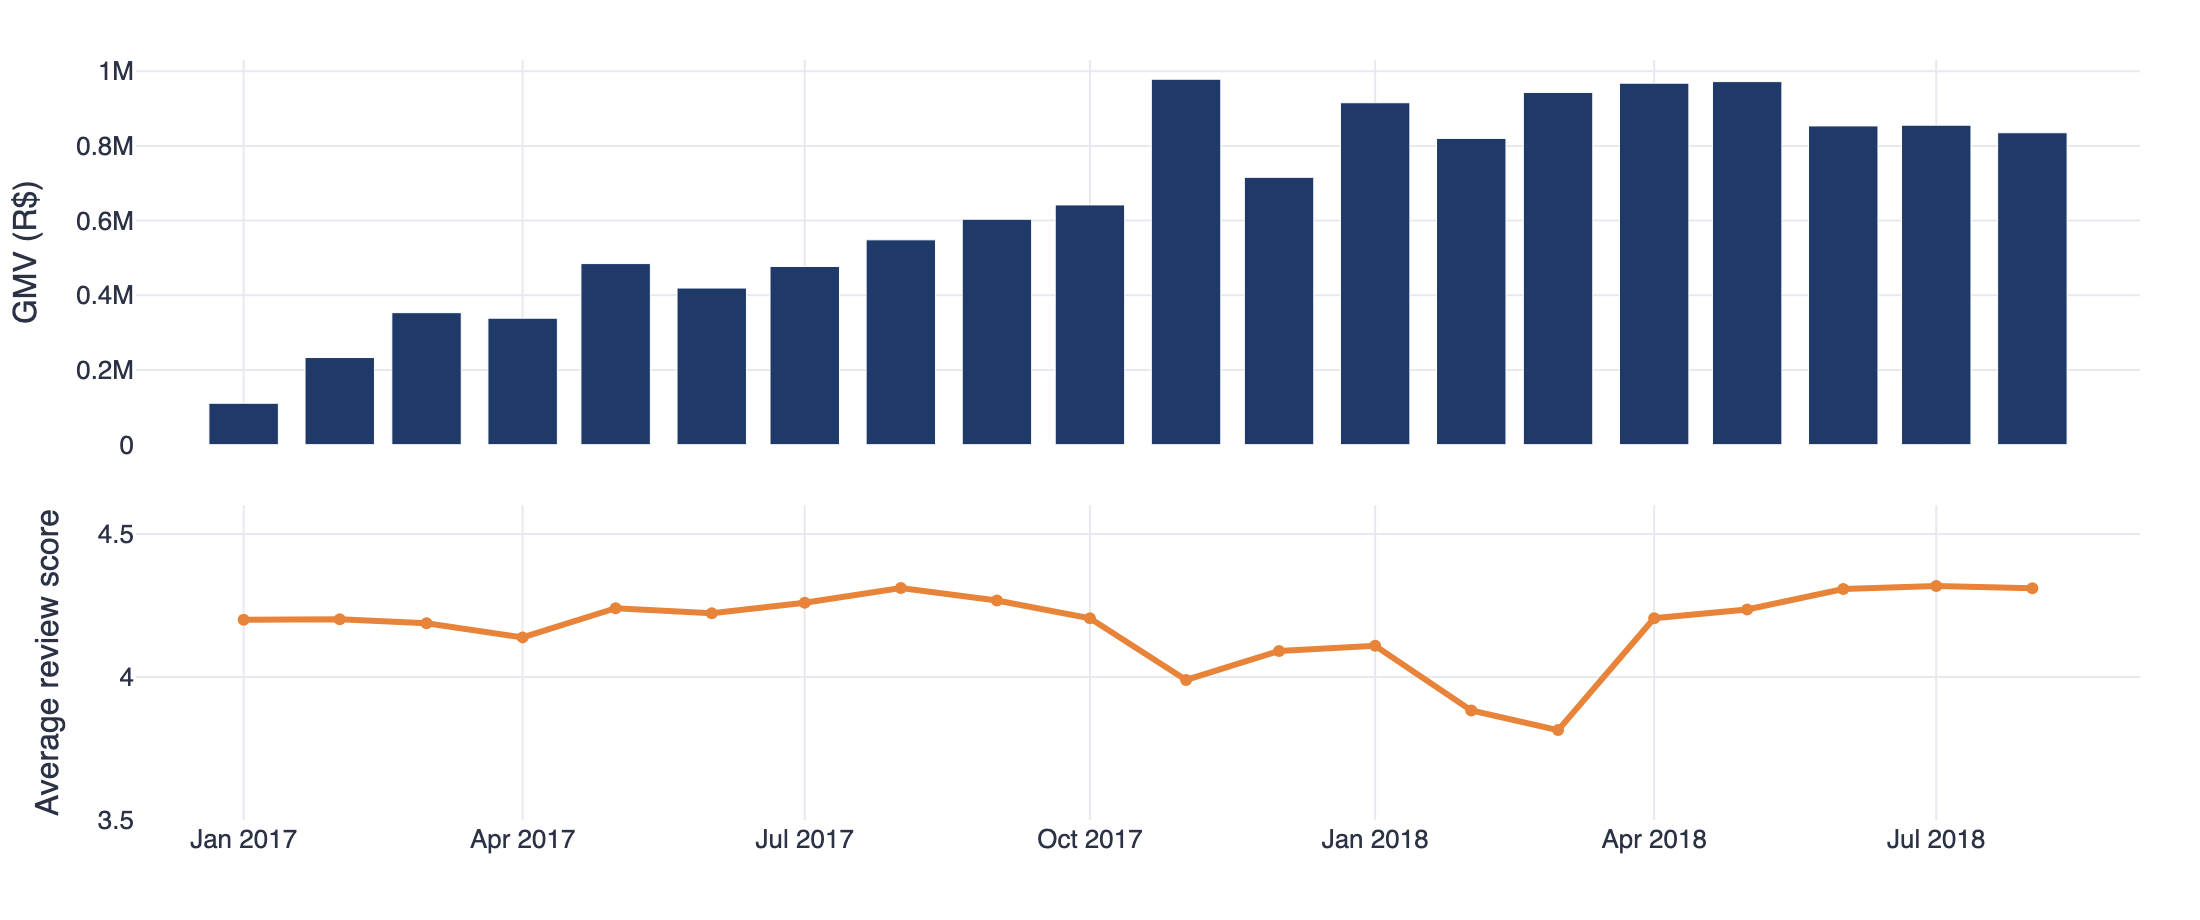
\includegraphics[width=0.92\textwidth]{01_growth_vs_satisfaction.png}
\caption{Monthly GMV and average review score. Presented as two aligned panels
sharing an axis rather than as a dual-axis chart, because the alignment between two
unrelated scales is arbitrary and can manufacture an apparent correlation.}
\label{fig:growth}
\end{figure}

We do not accept that reading. A national average spanning 27 states and roughly 70
product categories is a very blunt instrument and a flat line is precisely what
would be observed if one large healthy region masked several smaller failing ones.
S\~{a}o Paulo alone accounts for 42\% of orders. The appropriate response is not
reassurance but disaggregation, which motivates the segment analysis in
Section~\ref{sec:where}.

\subsection{The outcome variable}

The distribution of review scores is strongly bimodal: 59\% are five stars, 10\%
are one star and the entire two-to-three star band accounts for 11\%. The mean of
4.16 therefore describes a region in which relatively few observations actually
fall.

This shape determines the modelling approach. Predicting or tracking the mean score
is of limited operational value; what matters is whether an order produces a
\textbf{detractor}, defined as a review of one or two stars. That outcome is binary,
well defined and maps onto an action. It is used as the outcome variable
throughout.

%% ======================================================== 6
\section{Explanatory analysis}

\subsection{Lateness is a cliff, not a slope}

Orders delivered on time average 4.30 stars; orders delivered late average 2.57.
A difference of 1.73 stars from a single binary variable is larger than any other
effect we measured. 46\% of late orders receive a one-star review, against 7\% of
on-time orders.

The shape of that relationship matters more than its magnitude, because it
determines what an intervention should target (Figure~\ref{fig:cliff}).

\begin{figure}[H]
\centering
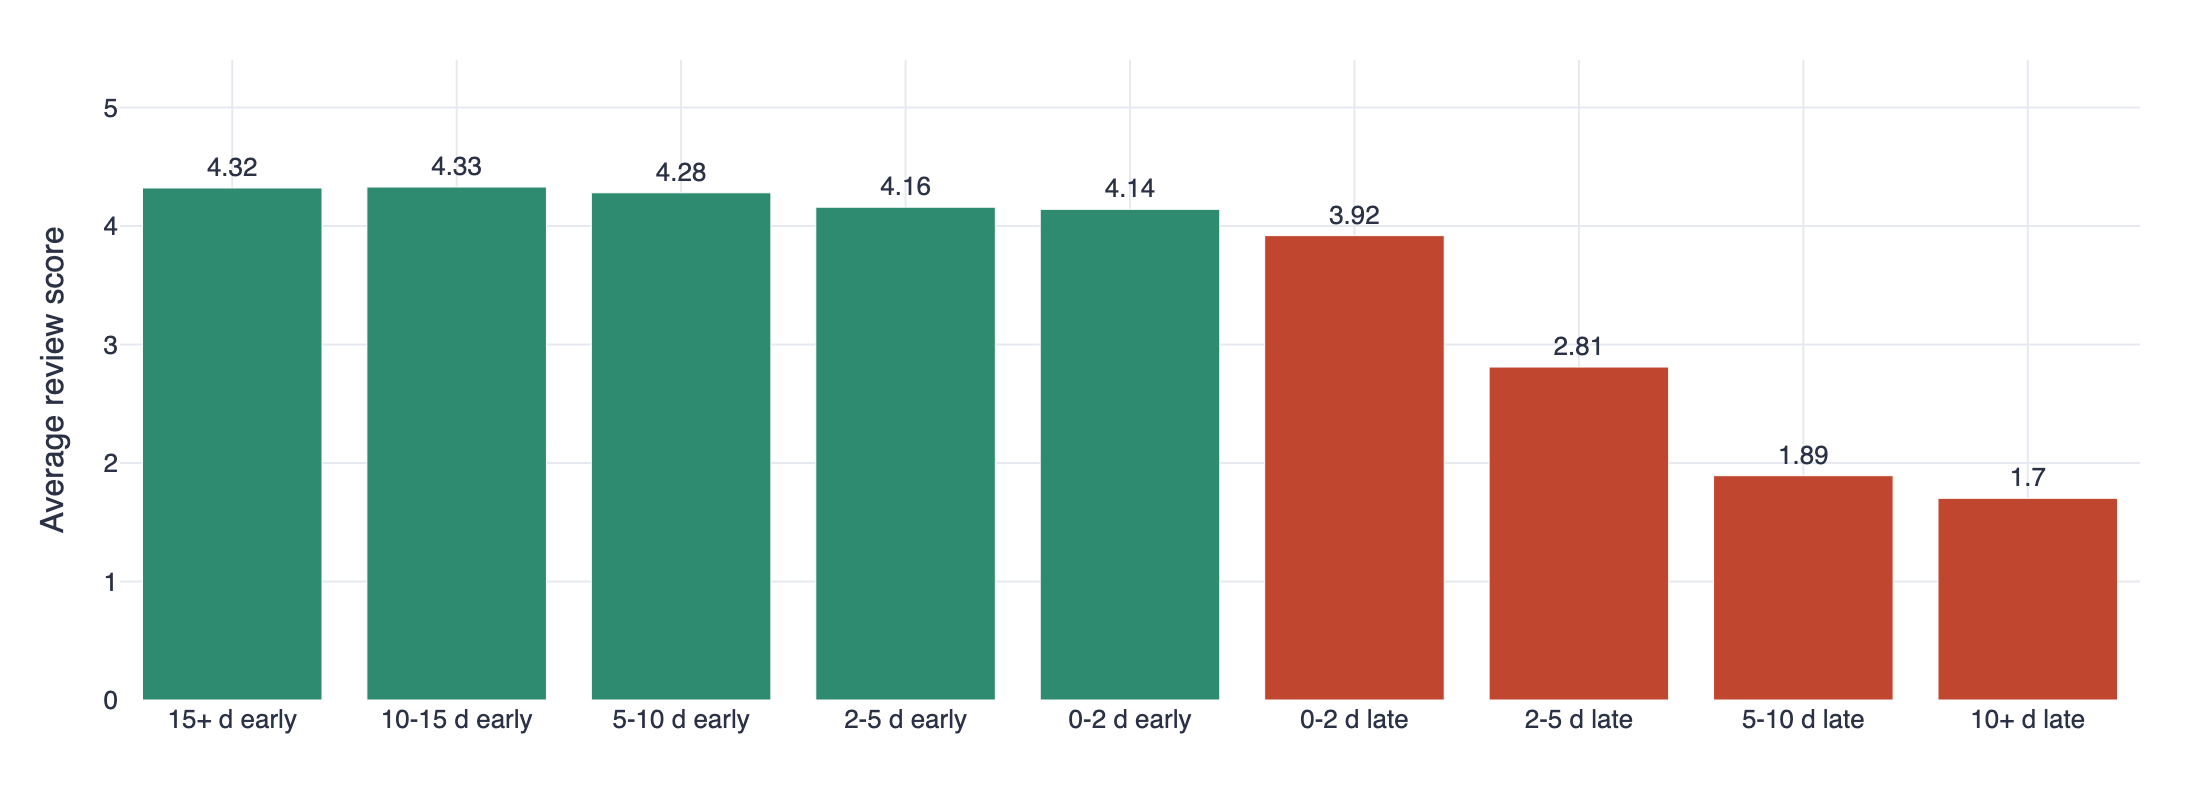
\includegraphics[width=0.92\textwidth]{03_delay_damage_curve.png}
\caption{Average review score by delivery timing relative to the promised date.}
\label{fig:cliff}
\end{figure}

\finding{Delivering fifteen days early (4.32) scores no better than delivering two
days early (4.14): once an order is comfortably inside its promise, additional
speed buys nothing. Past the promised date, the score falls from 3.92 at two days
late to 1.89 at five to ten days late. The damage is concentrated in the tail.}

The operational implication is specific and it changes what should be funded. The
objective is not to reduce average delivery time but to eliminate worst outcomes. A
programme shaving one day off every delivery nationally would achieve less than one
that repaired the slowest five percent.

\subsection{The delay belongs to the carrier}

The brief directs attention to slow sellers. This is the intuitive explanation and
it is also the lever the marketplace controls most directly. The stage decomposition
tests it (Figure~\ref{fig:journey}).

\begin{figure}[H]
\centering
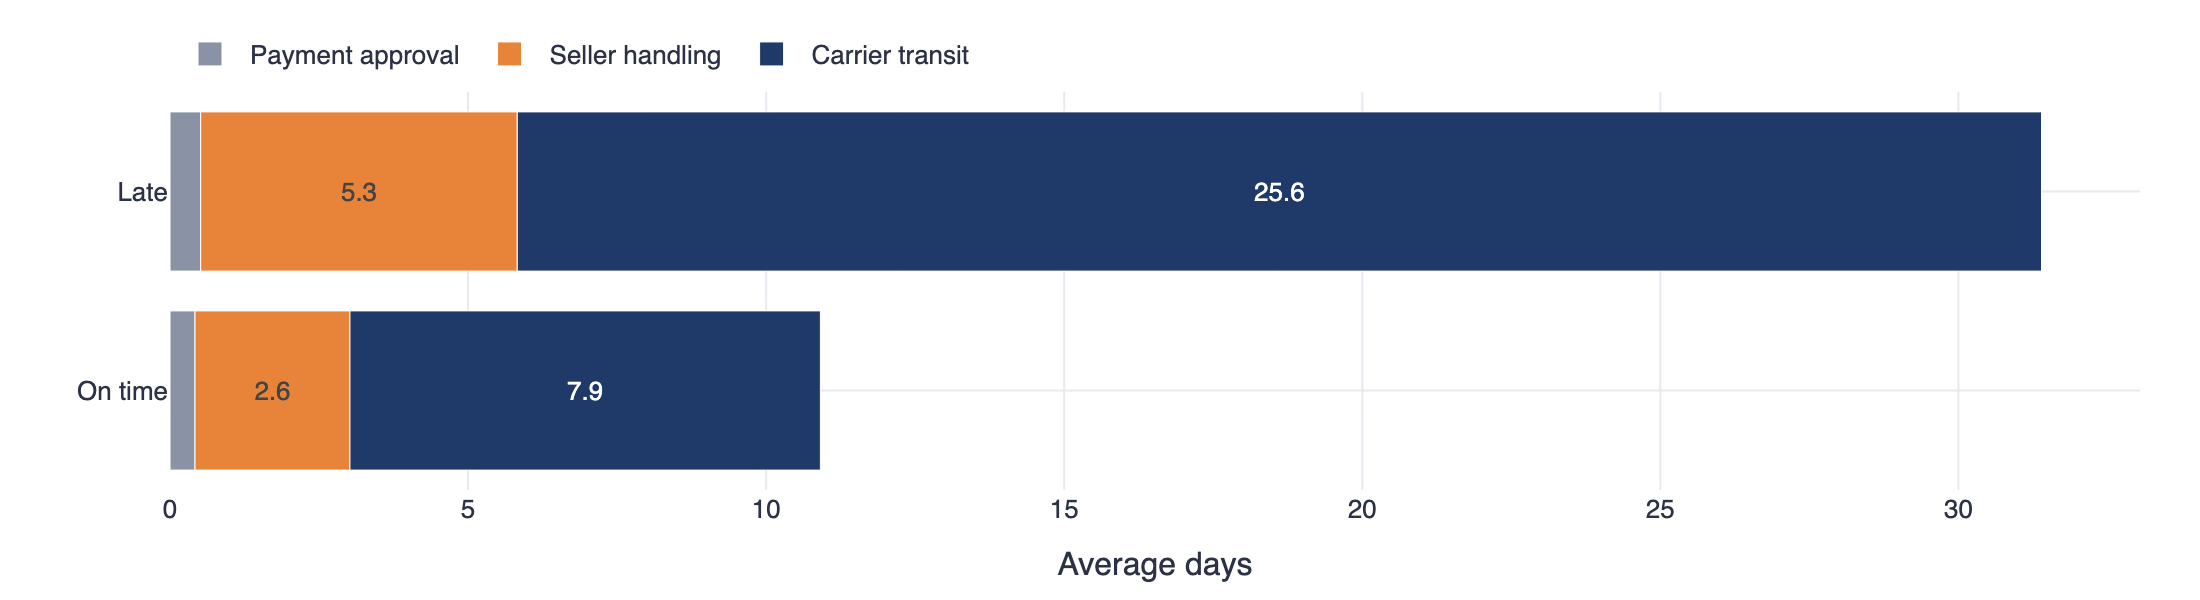
\includegraphics[width=0.88\textwidth]{04_journey_stages.png}
\caption{Where the days are spent, for on-time and late orders.}
\label{fig:journey}
\end{figure}

Sellers hand parcels to the carrier in 2.8 days on average; the carrier then holds
them for 9.3 days. On orders that end up late, the seller contributes 5.3 additional
days and the carrier 25.6. Correlation with the review score is $-0.16$ for seller
handling against $-0.30$ for carrier transit.

\finding{The carrier holds the parcel more than three times as long and correlates
with the outcome roughly twice as strongly. The intervention named in the brief is
aimed at the smaller half of the problem.}

This distinction is financially material, because coaching sellers and renegotiating
carrier contracts are different programmes with different budgets and different
owners.

\subsection{Independent verification}

The conclusion above is convenient, in the sense that a contrarian result is
rhetorically attractive and we treated that as a reason for additional scrutiny
rather than confidence. Before attaching a recommendation to it we sought evidence
from a source unrelated to delivery timestamps: the free-text review comments,
which are present on 41\% of reviews, written in Portuguese by customers
themselves.

Themes were assigned by keyword matching and cross-checked against a weighted
log-odds ranking with a Dirichlet prior, which identifies vocabulary distinctive of
negative reviews without being told in advance what to look for. The prior shrinks
small-sample terms toward zero, so surviving terms are both distinctive and well
evidenced.

\begin{table}[H]
\centering
\small
\caption{Themes in negative review comments ($n = 10{,}824$).}
\label{tab:themes}
\begin{tabular}{@{}lrr@{}}
\toprule
\textbf{Theme} & \textbf{Mentions} & \textbf{Share of negative comments}\\
\midrule
Delivery and lateness & 5{,}166 & 47.7\%\\
Order never arrived & 2{,}825 & 26.1\%\\
Refund or service response & 1{,}713 & 15.8\%\\
Wrong or missing item & 1{,}544 & 14.3\%\\
Product quality & 995 & 9.2\%\\
Damaged or defective & 589 & 5.4\%\\
\bottomrule
\end{tabular}
\end{table}

Nearly half of negative comments concern delivery and a quarter state that the
order never arrived, while product quality accounts for 9\%. The distinctive-term
ranking agrees: the strongest terms are \emph{recebi} (``I received''),
\emph{comprei} (``I bought''), \emph{pedido} (``order''), \emph{contato}
(``contact'') and two forms of the verb to wait. No term describing the product
itself appears near the top.

Two independent sources, structured timestamps and unstructured text, support the
same conclusion. One finding does not fit our recommendation and is reported
anyway: 15.8\% of complaints concern refunds and service response, which no
logistics investment addresses.

\subsection{Where the risk concentrates}
\label{sec:where}

Applying Satisfaction-at-Risk to shipping lanes localises the problem to a level at
which operations can act: a lane is a route and a contract, whereas a state is not
(Figure~\ref{fig:lanes}).

\begin{figure}[H]
\centering
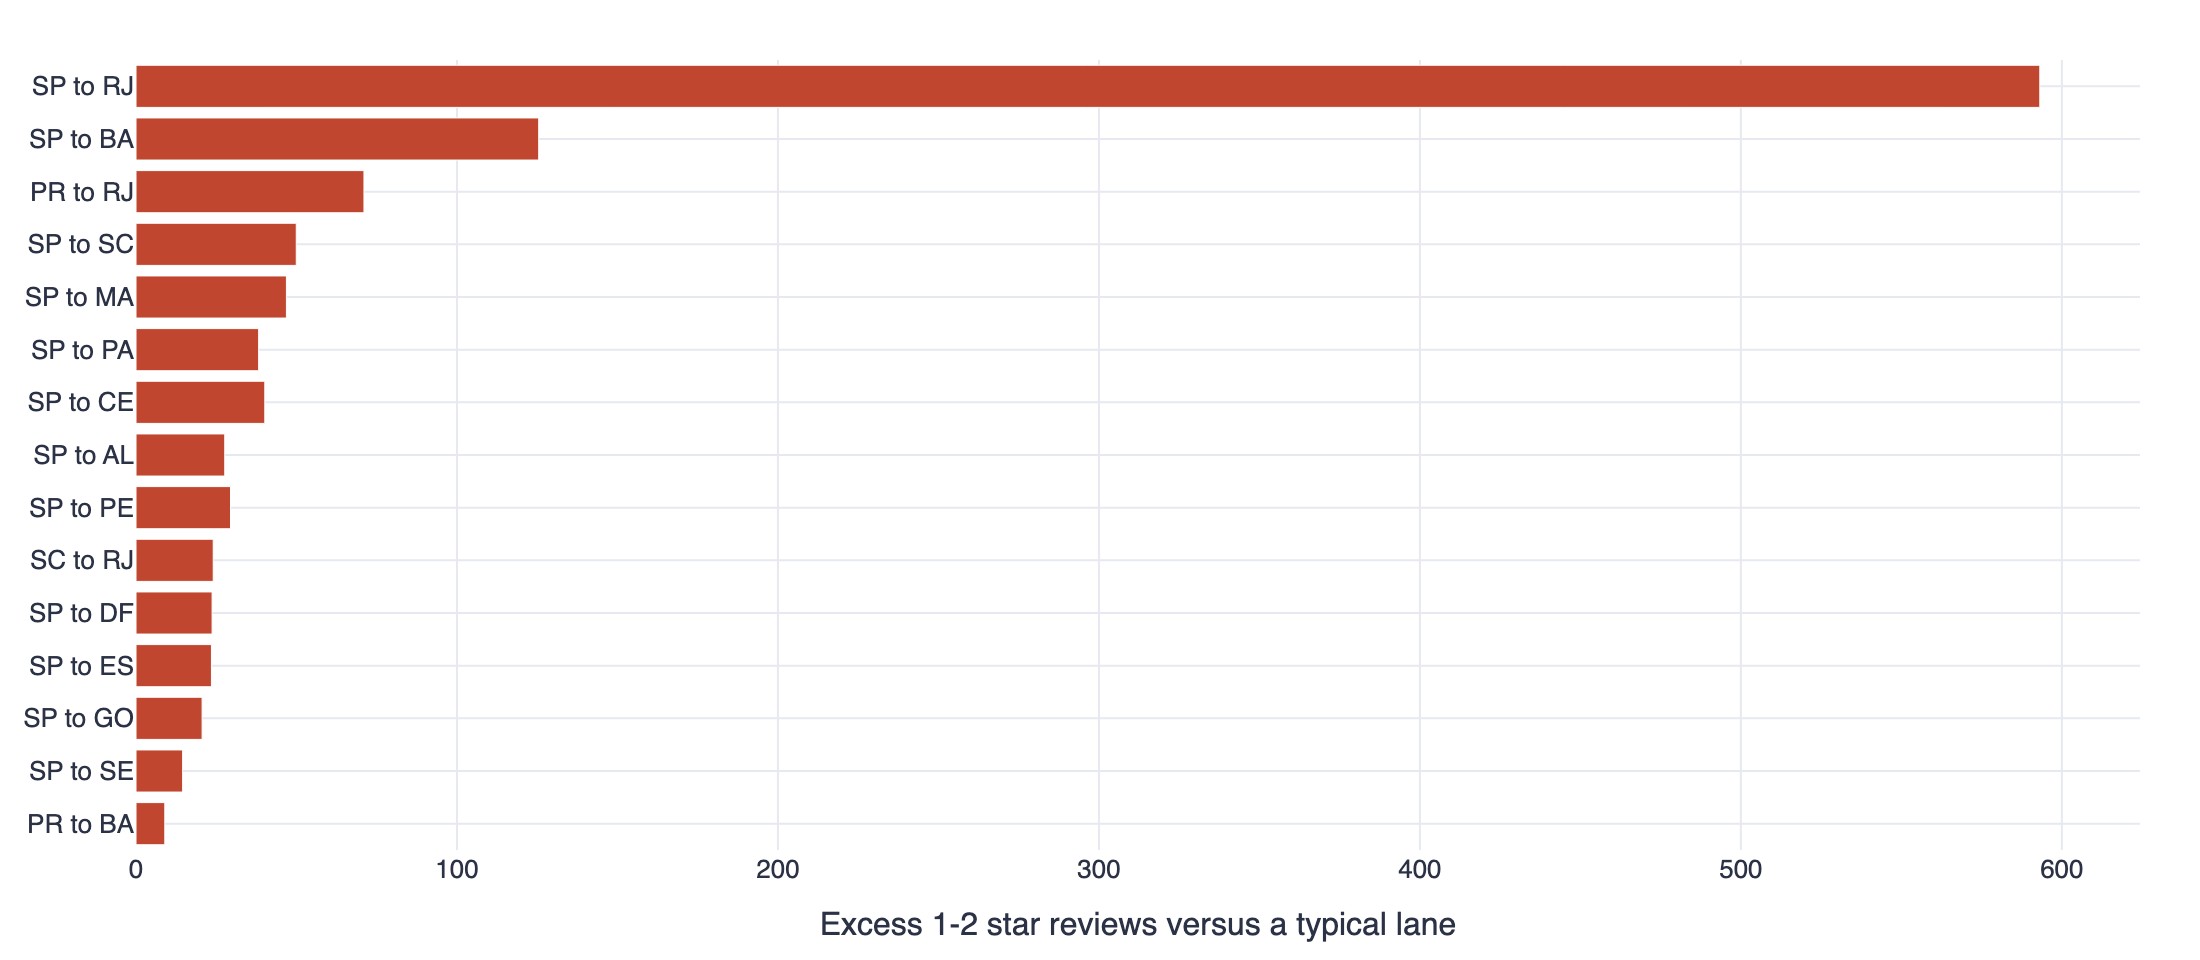
\includegraphics[width=0.88\textwidth]{09_lane_risk.png}
\caption{Excess detractors by origin--destination lane.}
\label{fig:lanes}
\end{figure}

\begin{table}[H]
\centering
\small
\caption{Regional performance for three contrasting states.}
\label{tab:states}
\begin{tabular}{@{}lrrrr@{}}
\toprule
\textbf{State} & \textbf{Orders} & \textbf{Avg. score} & \textbf{Late rate} & \textbf{Days to deliver}\\
\midrule
S\~{a}o Paulo & 40{,}171 & 4.25 & 5.8\% & 8.7\\
Rio de Janeiro & 12{,}172 & 3.96 & 13.3\% & 15.2\\
Maranh\~{a}o & 709 & 3.83 & 19.3\% & 21.5\\
\bottomrule
\end{tabular}
\end{table}

Rio de Janeiro is the state we would escalate and no league table sorted by average
score would surface it: 3.96 is unremarkable. It is the second-largest market in the
country and runs more than twice S\~{a}o Paulo's late rate, producing 678 excess
detractors, more than the next five states combined. S\~{a}o Paulo to Rio de Janeiro
is the single worst lane in the marketplace and it is a short-haul route between
neighbouring states, which suggests an operational fault rather than an unavoidable
consequence of geography.

\subsection{A structural effect with an unusually favourable ratio}

While testing whether basket composition affected satisfaction, expecting a null
result, we found the largest cheap win in the study. Orders filled by a single
seller average 4.17 stars; orders split across two sellers average 2.88; across
three or more, 2.24.

The mechanism is intuitive once stated. The customer places one order and receives
it in fragments over several days, waits for the slowest parcel and reviews the
entire order on that experience.

\finding{Split shipments cost approximately 1.3 stars and affect only 1.3\% of
orders. No other effect we measured has that ratio and unlike every other finding
in this report, addressing it requires no logistics expenditure: either consolidate
fulfilment or set per-parcel expectations at checkout.}

\subsection{The delivery promise is not slack}

The median order is promised in 23 days and arrives in 10. That apparent padding
invites trimming, which would improve checkout competitiveness at no operational
cost. We tested how much of it is genuinely spare by computing, per state, the
reduction that could be absorbed while still covering 92\% of orders, roughly the
current on-time rate.

The answer is very little. S\~{a}o Paulo carries 11.5 days of apparent padding of
which 1.7 days are safely removable; Rio de Janeiro, Rio Grande do Sul and Santa
Catarina have no safe margin at all. The padding is not waste but variance cover.
The median order does not require it; the 92nd-percentile order does and that is
precisely the order sitting on the cliff identified earlier.

%% ======================================================== 7
\section{Predictive modelling}

\begin{table}[H]
\centering
\small
\caption{Model performance on a temporally held-out test set ($n = 23{,}890$).}
\label{tab:model}
\begin{tabular}{@{}lrrrrr@{}}
\toprule
\textbf{Model} & \textbf{ROC AUC} & \textbf{PR AUC} & \textbf{Brier} &
\textbf{Top 10\% capture} & \textbf{Top 20\% capture}\\
\midrule
Post-hoc (includes outcome) & 0.727 & 0.337 & 0.078 & 37.2\% & 50.7\%\\
At-risk (checkout only) & 0.632 & 0.177 & 0.092 & 21.8\% & 35.7\%\\
\midrule
Baseline (base rate) & 0.500 & 0.100 & 0.091 & 10.0\% & 20.0\%\\
\bottomrule
\end{tabular}
\end{table}

An ROC AUC of 0.63 from checkout-time features is a modest result and we present
it as such rather than framing it favourably. We would argue it is the correct
modest result: a model reporting 0.9 on this task would almost certainly be using
information it should not have. Most of what makes a customer angry (a carrier
losing a parcel, a defective unit, an incorrect item) has not yet occurred when
the order is placed and is therefore not predictable in principle.

What the model does achieve is separation. The riskiest decile of orders contains
21.8\% of all eventual detractors and the riskiest quintile contains 35.7\%,
approximately twice the rate of random selection. That is sufficient to prioritise a
proactive outreach queue when only a fraction of orders can be reviewed.

\finding{The model ranks well but is not calibrated. Its Brier score of 0.0917 is
marginally worse than the base-rate baseline of 0.0913, meaning its probability
estimates are no better than predicting the marketplace average for every order.
It may be used to order a queue. It must not be used to quote a probability.}

This distinction is easy to lose and consequential: ROC AUC measures ranking, while
the Brier score measures whether the stated probabilities are honest. The
calibration curve confirms it visually, with predicted risk considerably flatter
than observed risk across deciles.

Comparing feature importance between the two models is the most informative result
in this section. The post-hoc model's second strongest feature is
\texttt{delay\_days}, which the at-risk model cannot access and that single absence
accounts for most of the gap between 0.73 and 0.63.

\finding{The variable that overwhelmingly determines customer satisfaction does not
exist at the moment of sale. It is created afterwards, by the carrier. This is the
central finding of the project expressed as a modelling result and it is why the
recommendations concern logistics rather than targeting or merchandising.}

%% ======================================================== 8
\section{Scenario simulation and recommendations}

\subsection{What each intervention costs}

\begin{table}[H]
\centering
\small
\caption{Simulated interventions, replayed against the observed order history.}
\label{tab:scenarios}
\begin{tabular}{@{}lrrrr@{}}
\toprule
\textbf{Scenario} & \textbf{Detractors avoided} & \textbf{GMV given up} &
\textbf{Late rate after} & \textbf{Net value}\\
\midrule
Do nothing & 0 & \R{}0 & 8.0\% & \R{}0\\
Fix the worst lanes & 835 & \R{}0 & 6.4\% & \R{}114{,}150\\
Remove the worst sellers & 400 & \R{}412{,}200 & 7.9\% & $-$\R{}357{,}496\\
Tighten the promise by 3 days & $-$1{,}639 & \R{}0 & 12.9\% & $-$\R{}224{,}221\\
Combined programme & 355 & \R{}412{,}200 & 9.1\% & $-$\R{}363{,}603\\
\bottomrule
\end{tabular}
\end{table}

\paragraph{The counter-intuitive result.} Shortening the delivery promise by three
days creates approximately 1{,}639 additional detractors and raises the late rate
from 8.0\% to 12.9\%. We expected the opposite. The padding is not sandbagging; it
is the only mechanism absorbing variance in a transit network that occasionally
takes a month. Removing it does not make orders slower, it reclassifies orders that
were quietly acceptable as officially late and the damage curve does the rest. The
correct sequencing follows directly: purchase the speed first, then spend it on a
shorter promise.

\paragraph{The unambiguous win.} Targeted investment in carrier speed on the worst
lanes avoids approximately 835 detractors at no revenue cost. It is the only lever
examined with unambiguously positive net value.

\subsection{Seller policy}

Every seller with at least 30 orders is scored on two independent axes: product
quality and delivery reliability. The 30-order threshold prevents a single
dissatisfied customer from determining a seller's fate.

\begin{table}[H]
\centering
\small
\caption{Seller verdicts. Shares are of total marketplace GMV.}
\label{tab:sellers}
\begin{tabular}{@{}lrr@{}}
\toprule
\textbf{Verdict} & \textbf{Sellers} & \textbf{GMV share}\\
\midrule
Invest: healthy on both axes & 439 & 51.6\%\\
Coach: fulfilment (good products, late) & 156 & 22.1\%\\
Coach: product quality (on time, poorly rated) & 4 & 1.8\%\\
Remove: fails both axes & 16 & 1.4\%\\
Monitor: fewer than 30 orders & 2{,}316 & 23.1\%\\
\bottomrule
\end{tabular}
\end{table}

The catalogue-shrinkage concern is largely unfounded at the irredeemable end. The
16 sellers failing on both axes hold 1.4\% of GMV; all could be delisted at a cost
of roughly one part in seventy of revenue. The larger and more interesting group is
the 156 sellers who deliver late while selling well-rated products. They represent
22\% of GMV and given the carrier finding, a substantial portion of their lateness
is not attributable to them. They require pickup scheduling and carrier support
rather than sanction.

\paragraph{Breakeven.} Delisting on the score axis alone removes 20 sellers, avoids
400 detractors and gives up \R{}412{,}200 of GMV. At an average order value of
\R{}136.76, delisting becomes profitable only if a lost customer is worth more than
\textbf{7.5 average orders} or approximately \R{}1{,}025. In a marketplace where
3.1\% of customers return, that threshold is unlikely to be met. We therefore
report the threshold rather than a verdict, but our reading is that coaching
dominates delisting for all but the 16 sellers failing on both axes.

\subsection{Recommendations}

\begin{enumerate}[leftmargin=*,itemsep=0.45em]
  \item \textbf{Fund carrier speed on the worst lanes.} The only intervention that
        improves experience at zero revenue cost. Begin with S\~{a}o Paulo to Rio
        de Janeiro, which is high-volume, short-haul and the worst-performing lane
        in the country.
  \item \textbf{Leave the delivery promise unchanged} until transit times have
        measurably fallen. It is protecting the on-time rate, not inflating a
        metric.
  \item \textbf{Coach 156 sellers and remove 16.} The removal list represents 1.4\%
        of GMV; the coaching list represents 22\%  and much of its lateness belongs
        to the carrier.
  \item \textbf{Address split shipments.} Approximately 1.3 stars lost on 1.3\% of
        orders, addressable through consolidated fulfilment or clearer per-parcel
        expectations at checkout. The cheapest item on this list.
  \item \textbf{Review the refund and service process.} 15.8\% of complaints,
        untouched by any logistics investment and owned by a different function.
\end{enumerate}

%% ======================================================== 9
\section{Limitations}

\paragraph{Lateness is treated as causal.} The relationship is steep, monotone and
independently corroborated by the review text, which is why we are comfortable
acting on it. Nonetheless some portion of the effect may proxy for correlated
failures such as poor seller communication. The scenario figures are magnitudes
rather than forecasts.

\paragraph{A detractor is valued at one average order.} A deliberate floor,
justified by the 3.1\% repeat-purchase rate. It excludes word-of-mouth effects
entirely, which is why the delisting decision is presented as a breakeven threshold
rather than a recommendation.

\paragraph{Removed sellers are treated as lost demand.} In practice a proportion of
those customers would be recaptured by other sellers on the platform, so the cost of
delisting presented here is a worst case.

\paragraph{The marketing funnel is incompletely observed.} 55\% of closed deals
belong to sellers who never transacted and therefore have no orders, reviews or
GMV. Channel-quality comparisons are correspondingly weak and we would not
reallocate budget on that table alone.

\paragraph{The data ends in October 2018.} Absolute levels have moved since. The
relationships between distance, lateness and satisfaction are considerably more
durable than the levels.

\paragraph{The single most valuable missing field is carrier identity.} It is absent
from the dataset and it would convert ``the carrier is slow'' into ``this carrier
is slow on this lane'', which is the difference between an observation and an
actionable instruction.

%% ======================================================== 10
\section{Technical appendix}
\label{sec:appendix}

\subsection{Repository structure}

\begin{table}[H]
\centering
\small
\caption{Repository layout.}
\label{tab:repo}
\begin{tabular}{@{}p{4.3cm}p{10.2cm}@{}}
\toprule
\textbf{Path} & \textbf{Contents}\\
\midrule
\texttt{src/} & The pipeline, one module per stage.\\
\texttt{app/streamlit\_app.py} & Interactive dashboard, six tabs.\\
\texttt{notebooks/} & Three narrative notebooks, one per project week.\\
\texttt{tests/test\_pipeline.py} & 22 tests covering ingest, features and analysis.\\
\texttt{outputs/tables/} & Computed aggregates consumed by every downstream artefact.\\
\texttt{reports/figures/} & Exported figures, PNG and interactive HTML.\\
\texttt{reports/} & Exported figures and this report's source.\\
\texttt{Makefile} & Reproducible build; \texttt{make all} runs the full pipeline.\\
\bottomrule
\end{tabular}
\end{table}

\subsection{Pipeline stages}

The build is a directed acyclic graph with a single entry point. Each stage writes
its outputs to disk and the next stage reads them, so any stage can be re-run in
isolation and intermediate results are inspectable.

\begin{table}[H]
\centering
\small
\caption{Pipeline modules, in execution order.}
\label{tab:modules}
\begin{tabular}{@{}p{3.3cm}p{11.2cm}@{}}
\toprule
\textbf{Module} & \textbf{Responsibility}\\
\midrule
\texttt{ingest.py} & Loads the eleven raw CSVs into DuckDB, deduplicates reviews,
clips out-of-range geolocation coordinates and produces the data quality audit.\\
\texttt{features.py} & Flattens the relational schema into one row per order,
constructs the stage durations and the distance estimate and runs sanity checks
before writing the fact table.\\
\texttt{analysis.py} & Defines the analysis population and the Satisfaction-at-Risk
metric; produces every aggregate table and the headline KPIs.\\
\texttt{model.py} & Fits the two classifiers with a temporal split and strictly
prior seller history; writes metrics, permutation importance and calibration.\\
\texttt{textmining.py} & Tokenises Portuguese review comments, computes weighted
log-odds with a Dirichlet prior and assigns complaint themes.\\
\texttt{simulate.py} & Fits the monotone delay--risk curve and replays the order
history under each scenario.\\
\texttt{export\_figures.py} & Renders every figure to PNG and interactive HTML.\\
\texttt{run\_notebooks.py} & Re-executes the three notebooks in place, refreshing
outputs while leaving the written narrative untouched.\\
\bottomrule
\end{tabular}
\end{table}

\subsection{Design decisions worth documenting}

\paragraph{One definition of the population.} \texttt{analysis\_base} is the only
place the analysis population is defined. Every figure, table, notebook and
dashboard tab calls it. This makes it structurally impossible for two outputs to
disagree about their denominator.

\lstinputlisting[caption={The single definition of the analysis population
(\texttt{src/analysis.py}).},firstline=29,lastline=40]{../src/analysis.py}

\paragraph{No downstream re-derivation.} The analysis layer computes each number
once and writes it to \texttt{outputs/tables/}. The dashboard, the notebooks and the
report all read those files rather than recomputing them. Any figure quoted in two
places therefore comes from a single calculation, which removes the most common way
for a set of deliverables to disagree with itself.

\paragraph{Leakage prevention is explicit.} Seller history is computed as an
expanding mean shifted by one order, so that an order can never contribute to the
feature used to predict it.

\lstinputlisting[caption={Strictly prior seller history
(\texttt{src/model.py}).},firstline=62,lastline=84]{../src/model.py}

\paragraph{One figure library.} Every chart in the report, the notebooks and the
dashboard is constructed in \texttt{src/viz.py}. The shared \texttt{style()} function
fixes typography, palette and background, which is why the three artefacts cannot
drift apart visually. Colour carries fixed meaning throughout: red denotes a bad
outcome, green a good one, amber attention and nothing is coloured decoratively.

\paragraph{Notebooks are executed, not generated.} The three notebooks are written
by hand and re-executed by \texttt{make all}. Code outputs are refreshed against the
current pipeline while the narrative is preserved, so quoted numbers cannot go stale
and prose cannot be overwritten.

\subsection{Reproducing this work}

\begin{lstlisting}[language=bash,caption={Full reproduction from raw data.}]
# 1. Place the eleven source CSVs in dashboard/data/raw/
# 2. From the dashboard/ directory:

python3 -m venv .venv && source .venv/bin/activate
make setup      # install dependencies from requirements.txt
make all        # ingest -> features -> analysis -> model ->
                # textmining -> figures -> notebooks
make test       # 22 tests covering the pipeline
make dash       # launch the dashboard on localhost:8501

tectonic reports/technical_report.tex # rebuild this document
\end{lstlisting}

The raw data is excluded from version control: the CSVs total approximately 120~MB
and the DuckDB build exceeds the hosting file-size limit. Everything else in the
repository is reproducible from those inputs.

\subsection{Testing}

The suite covers the properties that would silently corrupt results if violated:
that the analysis population is stable, that lateness is never coerced from null to
false, that order-level aggregates do not double-count multi-item orders, that
Satisfaction-at-Risk sums to approximately zero across a partition and that the
seller-history feature contains no future information.

%% ======================================================== 11
\section{Team contributions, work log and links}
\subsection{Team work distribution and track}
Each member maintained an individual work log for the duration of the project. The
table below summarises the division of responsibility; the detailed logs are
appended separately.

\begin{table}[H]
\centering
\small
\caption{Contribution summary.}
\label{tab:contrib}
\begin{tabular}{@{}p{3cm}p{5.4cm}p{6.4cm}@{}}
\toprule
\textbf{Member} & \textbf{Primary responsibility} & \textbf{Specific contributions}\\
\midrule
\lbrack Caleb, Hashir\rbrack& Data preparation and quality audit &
\lbrack Ingest, schema and grain verification, quality audit and treatments\rbrack\\
\addlinespace
\lbrack Karthik, Kautilya\rbrack& Exploratory analysis &
\lbrack Journey decomposition, geography and distance, structural effects\rbrack\\
\addlinespace
\lbrack Karthik, Caleb\rbrack& Explanatory visualisation &
\lbrack Figure library, colour system, damage curve and segment views\rbrack\\
\addlinespace
\lbrack All team members\rbrack& Modelling and simulation &
\lbrack Risk models, scenario engine, breakeven analysis\rbrack\\
\addlinespace
\lbrack All team members\rbrack& Dashboard and reporting &
\lbrack Streamlit console, technical report, final presentation\rbrack\\
\bottomrule
\end{tabular}
\end{table}

\begin{table}[H]
\centering
\small
\caption{Project timeline.}
\label{tab:timeline}
\begin{tabular}{@{}p{2.0cm}p{4.6cm}p{7.8cm}@{}}
\toprule
\textbf{Week} & \textbf{Focus} & \textbf{Output}\\
\midrule
Week 1 & Exploration and cleaning &
Schema and grain verified, quality audit completed, analysis population and
Satisfaction-at-Risk defined. Notebook 01.\\
\addlinespace
Week 2 & Exploratory and explanatory analysis &
All five questions answered, independent text verification completed, figure
library finalised. Notebook 02.\\
\addlinespace
Week 3 & Modelling, dashboard and delivery &
Risk models fitted, scenarios priced, dashboard built, report and presentation
produced. Notebook 03.\\
\bottomrule
\end{tabular}
\end{table}
\subsection{Links}
GitHub Repository: \href{}{}
\vspace{1.5em}
\noindent\textcolor{muted}{\small
All figures in this report were produced by the pipeline described in
Section~\ref{sec:appendix} and can be regenerated with \texttt{make all}. Numbers
quoted in the text are taken from \texttt{outputs/tables/} and were verified against
the executed notebooks at the time of writing.}


\end{document}
